%%%%%%%% AIMS-ICML 2023 style: Applied ML at Scale final report %%%%%%%%

\documentclass{article}

\usepackage{microtype}
\usepackage{graphicx}
\usepackage{subfigure}
\usepackage{booktabs}
\usepackage{hyperref}

\newcommand{\theHalgorithm}{\arabic{algorithm}}

\usepackage[accepted]{icml2023}

\usepackage{amsmath}
\usepackage{amssymb}
\usepackage{mathtools}
\usepackage{amsthm}
\usepackage{algorithm}
\usepackage{algorithmic}

\usepackage[capitalize,noabbrev]{cleveref}

\theoremstyle{plain}
\newtheorem{theorem}{Theorem}[section]
\newtheorem{proposition}[theorem]{Proposition}
\newtheorem{lemma}[theorem]{Lemma}
\newtheorem{corollary}[theorem]{Corollary}
\theoremstyle{definition}
\newtheorem{definition}[theorem]{Definition}
\theoremstyle{remark}
\newtheorem{remark}[theorem]{Remark}

\graphicspath{{figures/}}

\icmltitlerunning{Scaling ALS to 32 Million Ratings}

\begin{document}

\twocolumn[
\icmltitle{Scaling Alternating Least Squares to 32 Million Ratings:\\
Biases and Trait Vectors for Movie Recommendation}

\begin{icmlauthorlist}
\icmlauthor{Monzir Hafez}{aims}
\end{icmlauthorlist}

\icmlaffiliation{aims}{African Institute for Mathematical Sciences (AIMS) South Africa, 6 Melrose Road, Muizenberg 7975, Cape Town, South Africa}
\icmlcorrespondingauthor{Monzir Hafez}{monzir@aims.ac.za}

\icmlkeywords{Recommender Systems, Matrix Factorisation, Alternating Least Squares, MovieLens}

\vskip 0.3in
]

\printAffiliationsAndNotice{}

\begin{abstract}
We build a movie recommender on the full MovieLens 32M dataset, using
latent factor models fitted with Alternating Least Squares (ALS). Starting
from a probabilistic model, we derive closed-form ALS updates for a
biases-only model and for biased matrix factorisation with user and movie
trait vectors, and we show that no update can increase the regularised
loss. A compressed sparse row data layout and a parallel
compiled update kernel make training on all 32 million ratings practical
on a single CPU machine. With $K = 32$ latent dimensions the model reaches
a training RMSE of 0.605 and a test RMSE of 0.952 after 30 iterations. Its movie trait vectors
show genre structure that the model was never given, and folding in a new
user who rated a single film produces sensible recommendations. Our code is
available at \url{https://github.com/abualmun/als-project-notebook}.
\end{abstract}

\section{Introduction}
\label{sec:intro}

Recommender systems decide much of what people watch, read and buy online.
When a catalogue holds tens of thousands of items, no user can explore it
unaided, and a good system has to infer what a person will enjoy from very
little evidence about them. \emph{Collaborative filtering} addresses this
using only the record of past interactions between users and items. It
assumes that users who agreed in the past will tend to agree in the future,
and it learns that agreement directly from the data, without hand-crafted
item descriptions \cite{goldberg1992tapestry, sarwar2001item}.

Among collaborative filtering methods, \emph{latent factor models} became the
dominant approach after the Netflix Prize \cite{bennett2007netflix,
koren2009matrix}. These models map every user $m$ and every item $n$ to a
low-dimensional trait vector, $\mathbf{u}_m, \mathbf{v}_n \in \mathbb{R}^K$.
A rating is then explained by the inner product $\mathbf{u}_m^\top
\mathbf{v}_n$, plus a user bias and an item bias. This representation is
compact and easy to interpret, and it scales to very large data. With the
right choice of optimiser it can be trained on tens of millions of ratings on
a single machine.

In this report we build a movie recommendation prototype on the MovieLens
32M dataset \cite{harper2015movielens}, which contains 32 million ratings.
We derive every model from a regularised least-squares objective, fit it
with Alternating Least Squares (ALS) \cite{zhou2008large,
hu2008collaborative}, and evaluate it on a held-out test set. Our
contributions are as follows:
\begin{itemize}
  \item We plot the degree distributions of users and movies, which are
        heavy-tailed \cite{clauset2009power}.
  \item We derive closed-form ALS updates for a biases-only model and for the
        full model with biases and trait matrices $\mathbf{U}$ and
        $\mathbf{V}$, and we show that each update cannot increase the
        regularised loss.
  \item We describe an implementation that trains on all 32M ratings. It
        combines a compressed sparse row (CSR) data layout with a parallel
        just-in-time compiled update kernel \cite{lam2015numba}.
  \item We report train and test RMSE and loss curves, visualise the genre
        structure of the learned movie embeddings, and show recommendations
        for a ``dummy'' user who loves a single film.
\end{itemize}

The rest of the paper is organised as follows. \cref{sec:related} reviews
related work. \cref{sec:problem} states the problem and \cref{sec:data}
describes the dataset. \cref{sec:models} presents the models and their
derivations, and \cref{sec:implementation} covers the implementation at
scale. \cref{sec:results} reports our experiments, and
\cref{sec:conclusion} concludes.

\section{Related Work}
\label{sec:related}

\textbf{Collaborative filtering.}
Early recommender systems used neighbourhood methods. These predict a rating
from the ratings that similar users \cite{goldberg1992tapestry} or similar
items \cite{sarwar2001item} received. Neighbourhood methods are intuitive, but
they need a similarity matrix that grows with the number of users or items,
and they become unreliable when the data is sparse.

\textbf{Matrix factorisation.}
The Netflix Prize \cite{bennett2007netflix} established latent factor models
as the state of the art for rating prediction. \citet{koren2009matrix}
popularised the biased matrix factorisation model that we build on. In this
model, each rating is predicted from a user bias, an item bias, and the
inner product of user and item trait vectors, usually together with a
global offset. \citet{koren2008factorization} showed that neighbourhood and
latent factor views can be combined. \citet{salakhutdinov2008probabilistic}
gave the model a probabilistic interpretation, Probabilistic Matrix
Factorisation (PMF). Under PMF, the regularised squared-error loss is the
negative log posterior under Gaussian likelihoods and Gaussian priors. We
adopt this view throughout. It is what makes the regularisation strengths
interpretable as precisions, and it leads naturally to Bayesian treatments
of the same model \cite{salakhutdinov2008bayesian}.

\textbf{Alternating Least Squares.}
The matrix factorisation objective is not convex in $\mathbf{U}$ and
$\mathbf{V}$ jointly. However, it is a regularised least-squares problem in
either one when the other is held fixed. ALS exploits this by alternating
between exact solves for all users and exact solves for all items.
\citet{zhou2008large} used ALS with weighted regularisation on the Netflix
data and showed that it parallelises naturally, because every user (or
item) can be updated independently. \citet{hu2008collaborative} extended
ALS to implicit feedback. Unlike stochastic gradient descent, ALS has no
learning rate to tune. Each step also cannot increase the loss, which makes
monotone loss curves a useful check that an implementation is correct.

\textbf{Datasets.}
The MovieLens datasets \cite{harper2015movielens} are the standard public
benchmark for explicit-feedback recommendation. Like most interaction data,
their user and item degree distributions are heavy-tailed
\cite{clauset2009power}. This shapes both the statistical problem, because
many items have few ratings, and the engineering problem, because the
workload per user and per item is very uneven.

\section{Problem Statement}
\label{sec:problem}

We consider $M$ users, indexed by $m$, and $N$ movies, indexed by $n$. Their
interactions form a rating matrix $\mathbf{R} \in \mathbb{R}^{M \times N}$,
where $r_{mn} \in \{0.5, 1.0, \ldots, 5.0\}$ is the star rating that user $m$
gave movie $n$. Only a small fraction of the entries in $\mathbf{R}$ are
observed. We denote the set of observed user--movie pairs by
\begin{equation}
  \Omega = \{(m, n) : r_{mn} \text{ is observed}\}, \qquad |\Omega| \ll MN .
\end{equation}
Two views of $\Omega$ appear throughout the paper. The first is the set of
movies rated by user $m$, and the second is the set of users who rated
movie $n$:
\begin{equation}
  \Omega(m) = \{ n : (m, n) \in \Omega \}, \;\;
  \Omega(n) = \{ m : (m, n) \in \Omega \}.
\end{equation}
Their sizes, $|\Omega(m)|$ and $|\Omega(n)|$, are the \emph{degrees} of user
$m$ and movie $n$. Every ALS update in \cref{sec:models} reads exactly one
of these sets. In our implementation (\cref{sec:implementation}), each set
is a contiguous slice of an array.

\textbf{Task.}
We split $\Omega$ into disjoint sets $\Omega_{\text{train}}$ and
$\Omega_{\text{test}}$. Given only the ratings in $\Omega_{\text{train}}$, we
want a model that predicts a rating $\hat{r}_{mn}$ for any pair $(m, n)$. We
measure prediction accuracy with the root mean square error on a set
$\mathcal{S}$:
\begin{equation}
  \mathrm{RMSE}(\mathcal{S}) =
  \sqrt{\frac{1}{|\mathcal{S}|} \sum_{(m,n) \in \mathcal{S}}
  \left( r_{mn} - \hat{r}_{mn} \right)^2 } ,
  \label{eq:rmse}
\end{equation}
and we report it on both $\Omega_{\text{train}}$ and $\Omega_{\text{test}}$.
Training RMSE shows how well the model fits the data. Test RMSE estimates
how well it generalises, and the gap between the two indicates overfitting.

Low RMSE is not the final goal, however. A recommender must also rank the
whole catalogue for a given user. We therefore also judge the model
qualitatively, by whether the learned trait vectors give sensible
recommendations and a meaningful geometry of movies (\cref{sec:results}).

\section{Data}
\label{sec:data}

We use the MovieLens 32M dataset \cite{harper2015movielens}, collected by
the MovieLens movie recommendation service. Its users were selected at
random, and every selected user rated at least 20 movies. Ratings use a
five-star scale with half-star steps. Each movie in \texttt{movies.csv}
also carries a title and a pipe-separated list of genres.
\cref{tab:data} summarises the dataset as documented by its publishers.

\begin{table}[t]
\caption{MovieLens 32M as documented by GroupLens.}
\label{tab:data}
\vskip 0.15in
\begin{center}
\begin{small}
\begin{tabular}{lr}
\toprule
Ratings $|\Omega|$                 & 32{,}000{,}204 \\
Users $M$                          & 200{,}948 \\
Movies in the catalogue            & 87{,}585 \\
Rating scale                       & 0.5--5.0 stars \\
Minimum ratings per user           & 20 \\
\bottomrule
\end{tabular}
\end{small}
\end{center}
\vskip -0.1in
\end{table}

\textbf{Degree distributions.}
\cref{fig:powerlaw} plots how many users and how many movies have each
degree, computed on the first 100{,}000 rows of \texttt{ratings.csv}, the
subset used in our first, unoptimised implementation
(\cref{sec:implementation}). The file is ordered by user, so this subset
contains the complete rating histories of a small number of users with the
smallest ids. The movie degrees are heavy-tailed: almost 4{,}000 movies
have a single rating in this subset, while a few have more than 100, and
on log-log axes the frequencies fall close to a straight line over two
orders of magnitude, the signature of a power law
\cite{clauset2009power}. The user degrees span from 20 to almost 3{,}000
ratings, with most users at the low end. Because the subset holds few
users, each user degree occurs only a handful of times, so the user curve
is sparse. The single user with fewer than 20 ratings is the last one in
the subset, whose history is cut off by the 100{,}000-row limit.

This shape has two consequences. Statistically, many movies have too few
ratings to determine a $K$-dimensional trait vector from data alone, and it
is the prior (\cref{sec:models}) that keeps those vectors sensible.
Computationally, the work per user and per movie is very uneven, which
matters when the updates are parallelised (\cref{sec:implementation}).

\begin{figure*}[t]
\vskip 0.2in
\begin{center}
\centerline{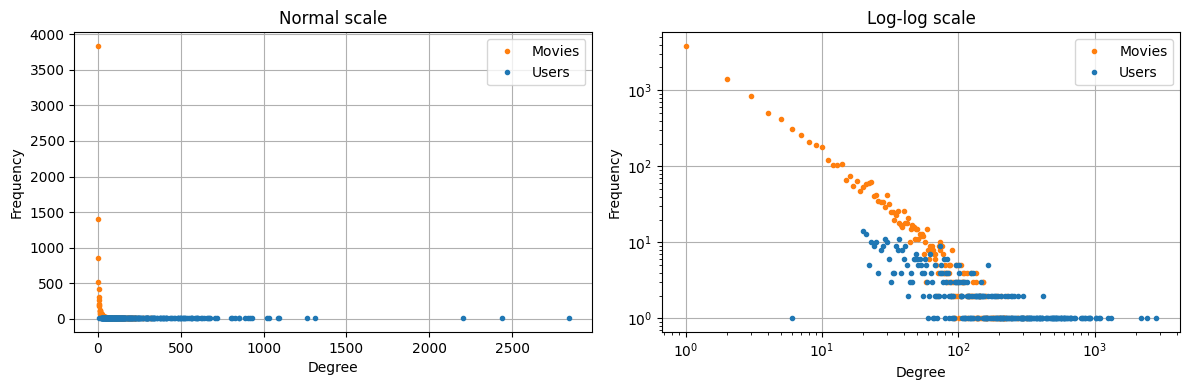
\includegraphics[width=0.85\textwidth]{fig_powerlaw}}
\caption{Degree distributions of users (blue) and movies (orange) on the
first 100{,}000 ratings of MovieLens 32M. Each point shows how many users
or movies have a given number of ratings. Left: linear axes. Right: log-log
axes.}
\label{fig:powerlaw}
\end{center}
\vskip -0.2in
\end{figure*}

\textbf{Train/test split.}
We split the ratings at random, at the level of individual ratings: each
rating is independently placed in $\Omega_{\text{train}}$ with probability
$0.8$ and in $\Omega_{\text{test}}$ otherwise. Because every user rated at
least 20 movies, almost every user keeps some ratings in the training set.
A rarely rated movie, however, can end up with all of its ratings in the
test set. Its bias and trait vector then stay at zero
(\cref{sec:mf}), so its predictions fall back on the user bias alone. We
keep such pairs in the test set rather than filtering them out, so the
reported test RMSE includes this cold-start penalty.

\section{Models}
\label{sec:models}

We study two nested models: per-user and per-movie biases
(\cref{sec:bias}), and biases plus latent trait vectors (\cref{sec:mf}).
Both are defined by a probabilistic generative model. Maximising its
posterior is equivalent to minimising a regularised squared-error loss, and
we minimise that loss with Alternating Least Squares. \cref{sec:foldin}
then shows how a trained model recommends movies to a user it has never
seen.

\subsection{Biases-only model}
\label{sec:bias}

The simplest useful model explains a rating by how generous the user is
and how good the movie is. We give each user a bias $b_m$ and each movie a
bias $c_n$, and we model
\begin{equation}
  r_{mn} = b_m + c_n + \epsilon_{mn}, \qquad
  \epsilon_{mn} \sim \mathcal{N}(0, \lambda^{-1}),
  \label{eq:bias-lik}
\end{equation}
with independent zero-mean Gaussian priors on the biases,
$b_m \sim \mathcal{N}(0, \gamma^{-1})$ and $c_n \sim \mathcal{N}(0, \gamma^{-1})$.
Here $\lambda$ is the precision of the rating noise and $\gamma$ is the prior
precision of the biases. The model has no separate global mean $\mu$.
Instead, the biases absorb the average rating, a choice we discuss below.

Taking the negative logarithm of the posterior, and dropping constants that
do not depend on the parameters, gives the loss
\begin{align}
  \mathcal{L}_{\text{bias}} = {}&
  \frac{\lambda}{2} \sum_{(m,n) \in \Omega_{\text{train}}}
  \left( r_{mn} - b_m - c_n \right)^2 \nonumber \\
  & + \frac{\gamma}{2} \sum_{m} b_m^2
  + \frac{\gamma}{2} \sum_{n} c_n^2 .
  \label{eq:loss-bias}
\end{align}
\cref{eq:loss-bias} is a convex quadratic in each bias on its own. Setting
$\partial \mathcal{L}_{\text{bias}} / \partial b_m = 0$ while holding all
the $c_n$ fixed gives the closed-form update
\begin{equation}
  b_m \leftarrow
  \frac{\lambda \sum_{n \in \Omega(m)} \left( r_{mn} - c_n \right)}
       {\lambda |\Omega(m)| + \gamma} ,
  \label{eq:bm-bias}
\end{equation}
and, by symmetry,
\begin{equation}
  c_n \leftarrow
  \frac{\lambda \sum_{m \in \Omega(n)} \left( r_{mn} - b_m \right)}
       {\lambda |\Omega(n)| + \gamma} .
  \label{eq:cn-bias}
\end{equation}
The full derivation is in \cref{app:bias}. Each ALS iteration applies
\cref{eq:bm-bias} to every user and then \cref{eq:cn-bias} to every movie.

These updates have a simple interpretation. Dividing the numerator and
denominator by $\lambda$ shows that $b_m$ is the average residual
$r_{mn} - c_n$ of user $m$, computed with $\gamma/\lambda$ extra
``pseudo-ratings'' of zero. A user with many ratings gets almost exactly
their empirical average. A user with very few ratings is shrunk towards
zero. The same holds for the movie biases, which are therefore a
regularised alternative to raw per-movie mean ratings, whose values are
noisy for movies with few ratings.

The same rescaling shows that the minimiser depends on the hyperparameters
only through the ratio $\gamma/\lambda$. Multiplying all precisions by a
common constant scales the loss but leaves its minimiser unchanged. We use
this fact when we discuss our choice of hyperparameters in
\cref{sec:setup}.

Without a global mean, the shrinkage pulls every bias towards zero rather
than towards the average rating. With $\gamma/\lambda = 0.5$, this costs
half a pseudo-rating per user or movie, and the effect is small for all but
the rarest movies. We keep the model in this form because it matches our
implementation exactly.

\subsection{Matrix factorisation with biases}
\label{sec:mf}

Biases alone cannot express taste: every user would receive the same
ranking of movies. To capture taste, we give each user a trait vector
$\mathbf{u}_m \in \mathbb{R}^K$ and each movie a trait vector
$\mathbf{v}_n \in \mathbb{R}^K$. Their inner product measures how well the
movie matches the user:
\begin{equation}
  r_{mn} = \mathbf{u}_m^\top \mathbf{v}_n + b_m + c_n + \epsilon_{mn},
  \qquad \epsilon_{mn} \sim \mathcal{N}(0, \lambda^{-1}) .
  \label{eq:mf-lik}
\end{equation}
Stacking the trait vectors as rows gives the matrices
$\mathbf{U} \in \mathbb{R}^{M \times K}$ and
$\mathbf{V} \in \mathbb{R}^{N \times K}$, so that
$\mathbf{R} \approx \mathbf{U}\mathbf{V}^\top$ plus biases. A low-rank
approximation of the rating matrix of this kind is what gives
matrix factorisation its name. We place isotropic Gaussian priors on the
traits, $\mathbf{u}_m \sim \mathcal{N}(\mathbf{0}, \gamma^{-1}\mathbf{I})$ and
$\mathbf{v}_n \sim \mathcal{N}(\mathbf{0}, \tau^{-1}\mathbf{I})$, and we keep
the bias priors from \cref{sec:bias}. The negative log posterior is then
\begin{align}
  \mathcal{L}_{\text{MF}} = {}&
  \frac{\lambda}{2} \sum_{(m,n) \in \Omega_{\text{train}}}
  \left( r_{mn} - \mathbf{u}_m^\top \mathbf{v}_n - b_m - c_n \right)^2
  \nonumber \\
  & + \frac{\gamma}{2} \sum_{m} \left( b_m^2 + \|\mathbf{u}_m\|^2 \right)
  \nonumber \\
  & + \frac{\gamma}{2} \sum_{n} c_n^2
  + \frac{\tau}{2} \sum_{n} \|\mathbf{v}_n\|^2 .
  \label{eq:loss-mf}
\end{align}
The user-side parameters share the precision $\gamma$, while the movie
traits have their own precision $\tau$. This lets us control how strongly
the movie vectors, which are the quantity we later interpret and visualise,
are shrunk.

\textbf{ALS updates.}
\cref{eq:loss-mf} is not convex in $(\mathbf{U}, \mathbf{V})$ jointly,
because of the product $\mathbf{u}_m^\top \mathbf{v}_n$. However, with all
movie parameters fixed, it is a strictly convex quadratic in each user's
bias and in each user's trait vector, and the reverse holds for the movie
parameters. For each user we first update the bias, using the current
trait vector:
\begin{equation}
  b_m \leftarrow
  \frac{\lambda \sum_{n \in \Omega(m)}
        \left( r_{mn} - \mathbf{u}_m^\top \mathbf{v}_n - c_n \right)}
       {\lambda |\Omega(m)| + \gamma} .
  \label{eq:bm-mf}
\end{equation}
Then, with the new bias, we define the residual
$y_{mn} = r_{mn} - b_m - c_n$ and set the gradient with respect to
$\mathbf{u}_m$ to zero. This gives a $K \times K$ linear system:
\begin{equation}
  \underbrace{\Big( \lambda \!\! \sum_{n \in \Omega(m)} \!\!
      \mathbf{v}_n \mathbf{v}_n^\top + \gamma \mathbf{I} \Big)}_{\mathbf{A}_m}
  \mathbf{u}_m
  = \underbrace{\lambda \!\! \sum_{n \in \Omega(m)} \!\! y_{mn} \mathbf{v}_n}_{\mathbf{d}_m} ,
  \label{eq:um}
\end{equation}
so that $\mathbf{u}_m \leftarrow \mathbf{A}_m^{-1} \mathbf{d}_m$.
The movie updates mirror \cref{eq:bm-mf,eq:um}. The roles of users and
movies are swapped, and $\tau$ replaces $\gamma$ in the trait system:
\begin{align}
  c_n &\leftarrow
  \frac{\lambda \sum_{m \in \Omega(n)}
        \left( r_{mn} - \mathbf{u}_m^\top \mathbf{v}_n - b_m \right)}
       {\lambda |\Omega(n)| + \gamma} ,
  \label{eq:cn-mf} \\
  \mathbf{v}_n &\leftarrow
  \Big( \lambda \!\! \sum_{m \in \Omega(n)} \!\!
      \mathbf{u}_m \mathbf{u}_m^\top + \tau \mathbf{I} \Big)^{-1}
  \lambda \!\! \sum_{m \in \Omega(n)} \!\! y_{mn} \mathbf{u}_m .
  \label{eq:vn}
\end{align}
The matrix $\mathbf{A}_m$ is a sum of positive semi-definite outer products
plus $\gamma\mathbf{I}$, so it is always positive definite and therefore
invertible. This holds even for a user with fewer than $K$ ratings, and even
for a movie with no training ratings at all. For such a movie,
\cref{eq:cn-mf,eq:vn} return $c_n = 0$ and $\mathbf{v}_n = \mathbf{0}$,
which is the cold-start behaviour described in \cref{sec:data}.
\cref{alg:als} summarises one training run.

\begin{algorithm}[tb]
  \caption{ALS for biased matrix factorisation}
  \label{alg:als}
\begin{algorithmic}
  \STATE {\bfseries Input:} $\Omega_{\text{train}}$, dimension $K$,
         precisions $\lambda, \gamma, \tau$, iterations $T$
  \STATE Initialise $b_m = c_n = 0$, and
         $\mathbf{u}_m, \mathbf{v}_n \sim \mathcal{N}(\mathbf{0}, K \mathbf{I})$
  \FOR{$t = 1$ {\bfseries to} $T$}
    \FOR{each movie $n$ {\bfseries in parallel}}
      \STATE Update $c_n$ by \cref{eq:cn-mf}, then $\mathbf{v}_n$ by \cref{eq:vn}
    \ENDFOR
    \FOR{each user $m$ {\bfseries in parallel}}
      \STATE Update $b_m$ by \cref{eq:bm-mf}, then $\mathbf{u}_m$ by \cref{eq:um}
    \ENDFOR
    \STATE Record $\mathcal{L}_{\text{MF}}$ and the train and test RMSE
  \ENDFOR
\end{algorithmic}
\end{algorithm}

\textbf{Monotone decrease and parallelism.}
Every step of \cref{alg:als} replaces one block of parameters with the exact
minimiser of $\mathcal{L}_{\text{MF}}$ over that block, holding the rest
fixed. The loss therefore can never increase from one step to the next.
Because it is bounded below by zero, the sequence of loss values converges
(\cref{app:monotone}). A monotonically decreasing loss curve is thus a
necessary check that the implementation is correct. Any increase points to
a bug rather than to a poorly tuned step size.

The same argument justifies parallelism. With $\mathbf{V}$ and $\mathbf{c}$
fixed, the parameters of different users appear in disjoint terms of
\cref{eq:loss-mf}. Updating all users at once therefore gives exactly the
same result as updating them one by one, and the same holds for movies.
This independence is what our parallel implementation exploits
(\cref{sec:implementation}).

\textbf{Non-identifiability.}
For any orthogonal matrix $\mathbf{Q}$, replacing
$\mathbf{u}_m \to \mathbf{Q}\mathbf{u}_m$ and
$\mathbf{v}_n \to \mathbf{Q}\mathbf{v}_n$ leaves every inner product, and
therefore the loss, unchanged. The isotropic priors are unchanged as well.
The learned trait space is therefore defined only up to a rotation or
reflection. When we visualise embeddings in \cref{sec:results}, the
\emph{relative} positions of movies carry meaning, but the individual axes
do not.

\textbf{Cost.}
Building $\mathbf{A}_m$ costs $\mathcal{O}(|\Omega(m)| K^2)$ and solving it
costs $\mathcal{O}(K^3)$. One full iteration therefore costs
$\mathcal{O}(|\Omega| K^2 + (M+N) K^3)$. The cost is linear in the number of
ratings, which makes training on all 32M ratings feasible.

\subsection{Recommending for a new user}
\label{sec:foldin}

At deployment time, a recommender must serve users who were not in the
training data. Retraining for every new user would be far too slow.
Instead, we \emph{fold in} the new user. We keep the movie parameters
$\mathbf{V}$ and $\mathbf{c}$ fixed and solve only for the new user's
$(b_\star, \mathbf{u}_\star)$, given their ratings. This is exactly the user
step of \cref{alg:als}, \cref{eq:bm-mf,eq:um}, applied to a single user and
started from $\mathbf{u}_\star = \mathbf{0}$. We repeat the bias and trait
updates five times. The procedure needs only the saved movie parameters,
so the training data never has to be loaded again.

To rank the catalogue, we score every movie $n$ by
\begin{equation}
  s_n = \mathbf{v}_n^\top \mathbf{u}_\star + w \, c_n ,
  \label{eq:score}
\end{equation}
and exclude the movies the user has already rated. The user bias $b_\star$
is the same for every movie, so it does not change the ranking and we drop
it. Setting $w = 1$ would rank movies by their predicted rating, in which
the movie bias, a measure of overall quality, counts as much as the match
with the user's taste. A small weight, $w = 0.05$, lets taste drive the
ranking while still favouring better movies among similar matches. Finally,
we exclude movies with fewer than a minimum number of training ratings,
because their trait vectors are determined mostly by the prior rather than
by data.

\section{Implementation at Scale}
\label{sec:implementation}

\cref{alg:als} is simple to write down, but a direct translation into
Python does not scale. Our first implementation stored the ratings as
Python lists of \texttt{(index, rating)} tuples, mapped raw string ids to
indices with dictionaries, and looped over the ratings one at a time,
inverting each $K \times K$ matrix explicitly. We used it only on the first
100{,}000 rows of \texttt{ratings.csv}. This section describes the changes
that make training on all 32M ratings practical on a single Google Colab
CPU instance: a new data layout, a new loading pipeline, and a compiled,
parallel update kernel.

\subsection{Compressed sparse row layout}
\label{sec:csr}

Every update in \cref{alg:als} reads exactly one of the sets $\Omega(m)$ or
$\Omega(n)$. We therefore store the training ratings twice, once grouped by
user and once grouped by movie. Each copy uses a compressed sparse row (CSR)
layout. For the user-grouped copy, we stable-sort the training triples
$(m, n, r_{mn})$ by user and keep two flat arrays: the movie indices
and the ratings, both of length $|\Omega_{\text{train}}|$. A pointer array
$\mathbf{p} \in \mathbb{N}^{M+1}$ holds the cumulative user training
degrees, with $p_0 = 0$ and $p_{m+1} = p_m + |\Omega(m)|$. The ratings of
user $m$ are then the contiguous slice
\begin{equation}
  \Omega(m) \;\leftrightarrow\; \big[\, p_m,\; p_{m+1} \big) ,
\end{equation}
which is read directly, without any search. The movie-grouped copy is built
in the same way. Storing the training data twice doubles its memory, but
both halves of each ALS iteration then read each user's or movie's ratings
from one contiguous block of memory instead of from scattered Python
objects.

\subsection{Memory-efficient loading}
\label{sec:loading}

In the first implementation, every rating created several Python objects:
a tuple in the per-user list, a tuple in the per-movie list, and a tuple in
each of the per-user and per-movie train or test lists. Our new loader
instead streams \texttt{ratings.csv} in chunks of two million rows with
\texttt{pandas}. Each chunk is parsed directly into typed NumPy arrays,
\texttt{int32} for ids and \texttt{float32} for ratings, so a rating
occupies 12 bytes. Raw MovieLens ids are not contiguous, so we map them to
dense indices $0, \ldots, M-1$ and $0, \ldots, N-1$ with a lookup table
rather than a dictionary. We mark which ids occur in a boolean array of
length $\max(\text{id}) + 1$, and the cumulative sum of this array gives
each present id its dense index. The train/test split (\cref{sec:data}) is
a vectorised Boolean mask on the flat arrays. Temporary arrays are deleted
as soon as they are no longer needed.

\subsection{Compiled, parallel ALS updates}
\label{sec:numba}

With the CSR layout, an intermediate version of our code performed each
user and movie update with vectorised NumPy operations on its slice, but
it still looped over all users and all movies in Python. Our final version
implements each half of \cref{alg:als} as a single kernel compiled to
machine code with Numba \cite{lam2015numba}. The same kernel serves both
halves, because the user and movie updates differ only in which CSR copy,
which fixed parameters and which precision they receive.

The kernel exploits three properties of the problem.
\begin{enumerate}
  \item \textbf{Parallelism.} Updates to different users are independent
        (\cref{sec:mf}), so the outer loop runs as a parallel loop
        (\texttt{prange}) across all CPU cores, with no locking. The same
        holds for movies.
  \item \textbf{Symmetry.} The matrix $\mathbf{A}_m$ in \cref{eq:um} is
        symmetric. We accumulate only its upper triangle and mirror it
        afterwards, which roughly halves the
        $\mathcal{O}(|\Omega(m)|K^2)$ cost of building it.
  \item \textbf{No intermediate arrays.} The bias update and the
        construction of $\mathbf{A}_m$ and $\mathbf{d}_m$ are plain loops
        over the slice of $\Omega(m)$. No arrays of size $|\Omega(m)|$
        are allocated, which matters for the most active users and the
        most popular movies.
\end{enumerate}
The trait vector is then obtained by solving the $K \times K$ system with
\texttt{np.linalg.solve}. We never form the explicit inverse
$\mathbf{A}_m^{-1}$, which would be slower and less numerically stable. The
kernel is compiled with Numba's \texttt{parallel} and \texttt{fastmath}
options.

To evaluate the loss and the RMSE, we compute predictions with a batched
\texttt{einsum} over blocks of one million ratings, which bounds the memory
needed for the gathered trait vectors.

\section{Experiments and Results}
\label{sec:results}

\subsection{Experimental setup}
\label{sec:setup}

\begin{figure*}[t]
\vskip 0.2in
\begin{center}
\centerline{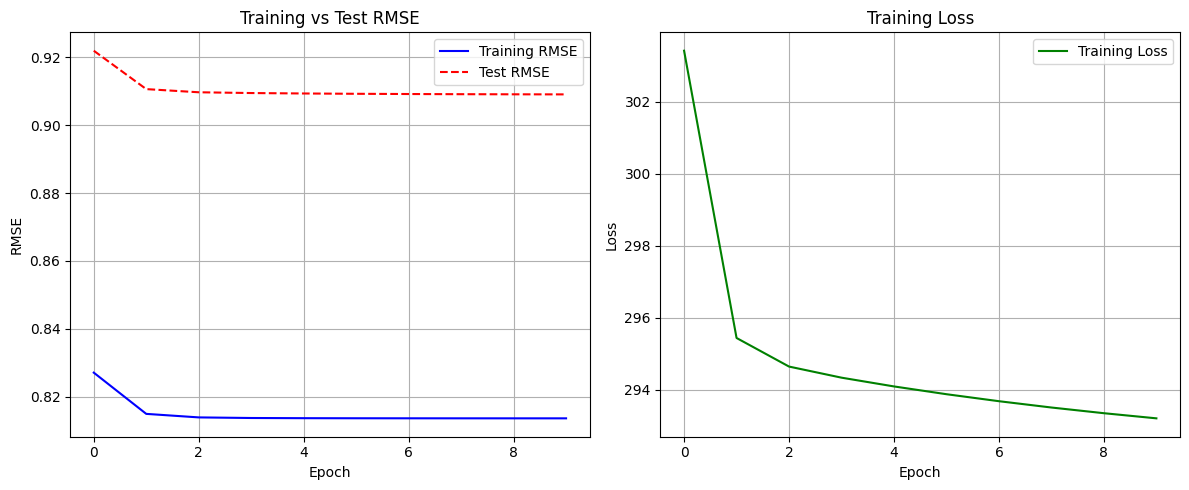
\includegraphics[width=0.8\textwidth]{fig_curves_bias}}
\vskip 0.1in
\centerline{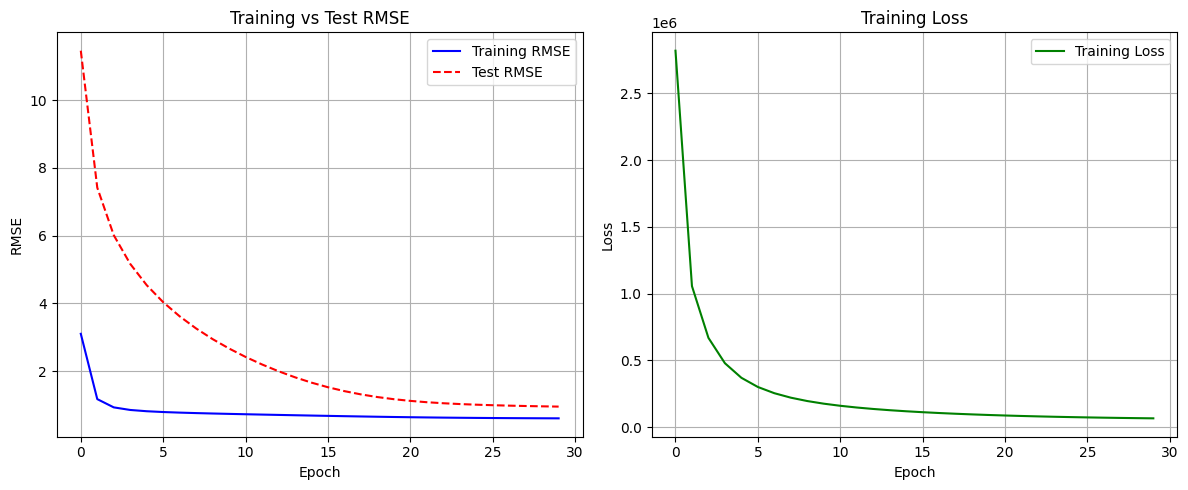
\includegraphics[width=0.8\textwidth]{fig_curves_mf}}
\caption{Training curves. Top: biases-only model on the first 100{,}000
ratings, with the regularised loss $\mathcal{L}_{\text{bias}}$
(\cref{eq:loss-bias}). Bottom: biased matrix factorisation with $K = 32$ on
all 32M ratings, with the regularised loss $\mathcal{L}_{\text{MF}}$
(\cref{eq:loss-mf}). In each row, the left panel shows train (solid) and
test (dashed) RMSE per ALS iteration and the right panel shows the loss.}
\label{fig:curves}
\end{center}
\vskip -0.2in
\end{figure*}

\begin{figure}[!t]
\vskip 0.2in
\begin{center}
\centerline{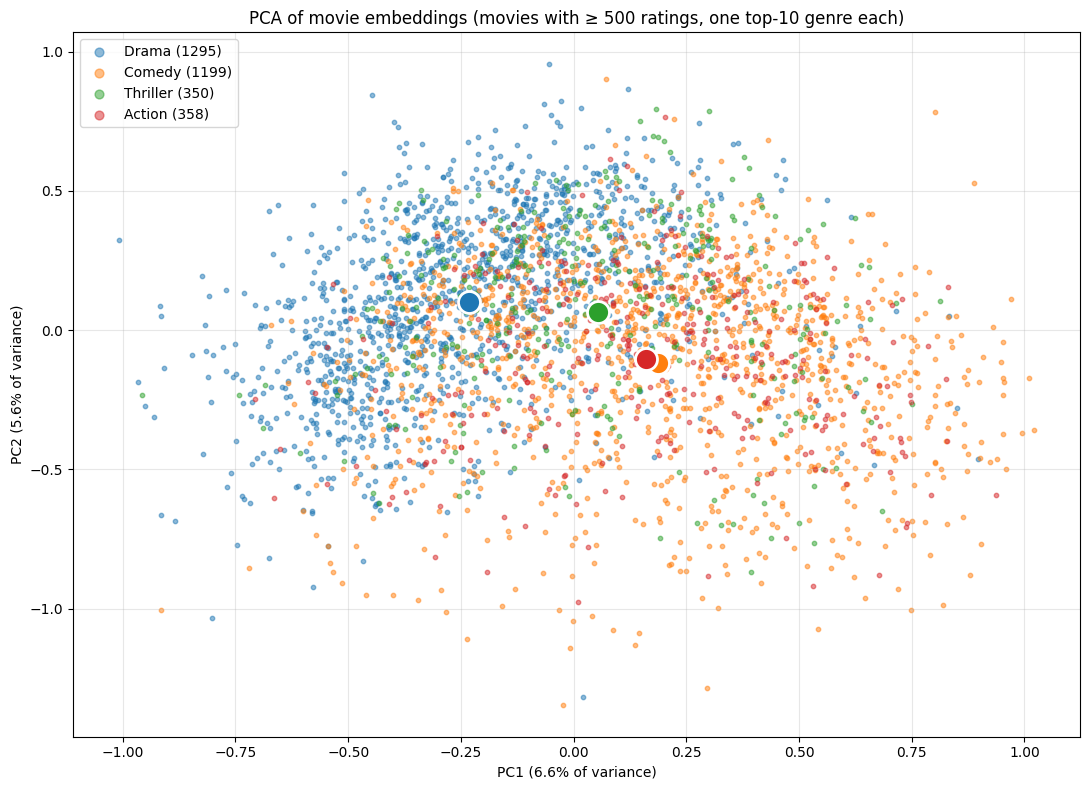
\includegraphics[width=\columnwidth]{fig_pca_genres}}
\caption{First two principal components of the $K = 32$ movie trait
vectors, for movies with $\geq 500$ training ratings that belong to exactly
one of the most common genres. The number of movies in each group is given
in the legend. Large dots are genre centroids.}
\label{fig:pca}
\end{center}
\vskip -0.2in
\end{figure}







We train the biases-only model with our first implementation on the first
100{,}000 rows of \texttt{ratings.csv}, and the full model with the Numba
implementation on all 32M ratings. Each run uses its own random 80/20
split (\cref{sec:data}), so the RMSE values of the two models are not
directly comparable. The embedding and recommendation results come from
the movie parameters $\mathbf{V}$ and $\mathbf{c}$ of the full model,
which we save to disk together with each movie's number of training
ratings.

\textbf{Hyperparameters.}
We use $\lambda = 0.01$, $\gamma = 0.005$ and $\tau = 0.01$ for both models,
and $K = 32$ latent dimensions for the full model. As shown in
\cref{sec:bias}, the minimiser depends only on the ratios
$\gamma/\lambda = 0.5$ and $\tau/\lambda = 1$. Each bias is therefore shrunk
as if it had half an extra rating of zero, and each movie trait vector is
shrunk with the strength of one extra observation. For any movie with more
than a handful of ratings, the data term dominates the prior.

\textbf{Initialisation and iterations.}
All biases start at zero. In the full model, trait vectors are drawn from
$\mathcal{N}(\mathbf{0}, K\mathbf{I})$, so for $K = 32$ each coordinate has
standard deviation $\sqrt{32} \approx 5.7$. We train the biases-only model
for 10 iterations and the full model for 30.

\subsection{Biases-only model}
\label{sec:res-bias}

\cref{fig:curves} (top) shows the training loss and the train and test RMSE
of the biases-only model on the 100{,}000-rating subset. Both RMSE curves
drop after the first iteration and are flat from the second iteration
onwards, ending at a train RMSE of about 0.81 and a test RMSE of about
0.91 (\cref{tab:rmse}). The loss decreases at every iteration, from about
303 to about 293. The model has only one parameter per user and per movie,
so the gap between train and test RMSE stays small.



\subsection{Matrix factorisation with biases}
\label{sec:res-mf}



\cref{fig:curves} (bottom) shows the training curves of the full model with
$K = 32$ on all 32M ratings. The regularised loss decreases at every
iteration, as \cref{app:monotone} guarantees, from $2.82 \times 10^{6}$
after the first iteration to $6.64 \times 10^{4}$ after the thirtieth.
After the first iteration the train and test RMSE are 3.10 and 11.46:
the broad initialisation leaves predictions far outside the rating scale,
and the movie traits, which are updated first, are fitted to random user
vectors. The train RMSE falls below 1 by the third iteration and reaches
0.605 after 30 iterations. The test RMSE falls more slowly, reaching 0.952
(\cref{tab:rmse}). It was still decreasing when training stopped, by 0.008
between the last two iterations, so more iterations would lower it
further.

The gap between train and test RMSE, 0.605 against 0.952, is much larger
than in the biases-only model. With $K = 32$, each user and movie has 33
free parameters, and the weak prior ($\tau/\lambda = 1$) lets movies and
users with few ratings fit their training ratings closely.





\begin{table}[t]
\caption{Final RMSE of the two models. Each model uses its own random
80/20 split of the data shown. The biases-only values are read from
\cref{fig:curves} (top).}
\label{tab:rmse}
\vskip 0.15in
\begin{center}
\begin{small}
\begin{tabular}{llrrr}
\toprule
Model & Data & Iter. & Train & Test \\
\midrule
Biases only        & 100K & 10 & $\approx$0.81 & $\approx$0.91 \\
Biases + traits    & 32M  & 30 & 0.605 & 0.952 \\
\bottomrule
\end{tabular}
\end{small}
\end{center}
\vskip -0.1in
\end{table}

\subsection{Genre structure of the movie embeddings}
\label{sec:res-embed}

To visualise the 32-dimensional trait space, we project the vectors
$\mathbf{v}_n$ of all movies with at least 500 training ratings onto their
first two principal components. Restricting to well-rated movies matters,
because the trait vectors of rarely rated movies are determined mostly by
the prior rather than by data. Among these movies the most common genres
are Drama (2{,}585 movies), Comedy (2{,}060), Thriller
(1{,}365) and Action (1{,}287). The first two components explain only
6.6\% and 5.6\% of the variance, so the projection is a thin slice of the
trait space. Because the space is defined only up to rotation
(\cref{sec:mf}), only the relative positions of movies carry meaning.

\cref{fig:pca} colours the projection by genre. We find the ten most common
genres among the projected movies, ignoring the ``IMAX'' and ``no genres
listed'' tags, and keep only movies that belong to exactly one of these
genres, so that each point has a single unambiguous colour. Large dots mark each genre's
centroid. The figure shows four groups: Drama (1{,}295
movies), Comedy (1{,}199), Action (358) and Thriller (350). The groups
overlap heavily, but they are not placed at random. Drama movies lie mostly
on the left of the first principal component and Comedy movies mostly on
the right, so their centroids are clearly apart along PC1. The Action
centroid lies next to the Comedy centroid, and the Thriller centroid lies
between the Drama and Action centroids. The model was never given genre
labels, so this separation emerges purely from rating patterns.



\subsection{Recommendations for a new user}
\label{sec:res-recs}

We create a dummy user who has rated a single movie, \emph{The Lord of the
Rings: The Fellowship of the Ring} (2001), with five stars. We fold this
user into the saved $K = 32$ model (\cref{sec:foldin}) and rank all movies
with at least 500 training ratings using \cref{eq:score} with $w = 0.05$.
\cref{tab:recs} lists the top ten.

\begin{table*}[t]
\caption{Top-10 recommendations for a dummy user who rated \emph{The
Fellowship of the Ring} five stars ($K = 32$, $w = 0.05$, movies with
$\geq 500$ training ratings).}
\label{tab:recs}
\vskip 0.15in
\begin{center}
\begin{small}
\begin{tabular}{rlrr}
\toprule
\# & Title & Score & Ratings \\
\midrule
1  & LOTR: The Return of the King (2003)  & 0.832 & 54{,}004 \\
2  & LOTR: The Two Towers (2002)          & 0.824 & 53{,}747 \\
3  & The Hobbit: An Unexpected Journey (2012)  & 0.616 & 12{,}935 \\
4  & The Hobbit: The Desolation of Smaug (2013) & 0.608 & 9{,}697 \\
5  & The Hobbit: The Battle of the Five Armies (2014) & 0.590 & 6{,}862 \\
6  & Hamilton (2020)                       & 0.485 & 1{,}524 \\
7  & The Thin Red Line (1998)              & 0.462 & 7{,}613 \\
8  & Evangelion: 2.0 You Can (Not) Advance (2009) & 0.438 & 629 \\
9  & Evangelion: 1.0 You Are (Not) Alone (2007)   & 0.434 & 683 \\
10 & Pride and Prejudice (1995)            & 0.419 & 2{,}463 \\
\bottomrule
\end{tabular}
\end{small}
\end{center}
\vskip -0.1in
\end{table*}

The seed movie has 58{,}427 training ratings. The two other Lord of the
Rings films are ranked first and second, well ahead of the rest, and the
three Hobbit films, prequels set in the same world, follow in third to fifth place. The remaining five are more
varied: a musical, a war film, two anime films and a period drama. Their
scores are lower, between 0.42 and 0.49. Two of them have fewer than 700
training ratings, close to the 500-rating cut-off, where trait vectors are
less well determined.
A single rating is enough to produce a meaningful user vector. With one
rating, \cref{eq:um} gives $\mathbf{u}_\star$ as a scaled copy of
$\mathbf{v}_{\text{LOTR}}$, so the ranking is driven by the inner product
$\mathbf{v}_n^\top \mathbf{v}_{\text{LOTR}}$: it returns the movies whose
trait vectors, learned from the ratings of all training users, point in the
same direction as that of \emph{The Fellowship of the Ring}.

\section{Conclusion}
\label{sec:conclusion}

We built a movie recommendation prototype on all 32 million ratings of
MovieLens 32M. Starting from a probabilistic model, we derived closed-form
ALS updates for a biases-only model and for biased matrix factorisation.
Every update is an exact block minimisation, so the regularised loss
decreases monotonically. A CSR data layout and a parallel compiled kernel
made training on the full dataset practical on a single CPU machine. With
$K = 32$, the model reached a test RMSE of 0.952 after 30 iterations, its movie
embeddings show genre structure that emerged from ratings alone, and a
single five-star rating was enough to produce recommendations for a new
user.

\textbf{Limitations.}
We evaluated on a random split at the level of ratings, with no separate
validation set. The model has no global mean, so all biases are shrunk
towards zero instead of towards the average rating. Users choose which
movies to rate, so the observed ratings are not missing at random, and
RMSE on held-out observed ratings says little about movies that users never
chose to watch. Finally, all our estimates are point estimates and carry no
measure of uncertainty.

\textbf{Future work.}
A Variational Bayes treatment of $\mathbf{U}$, $\mathbf{V}$ and the biases
would replace the point estimates with posterior distributions, giving
uncertainty estimates that matter most for the long tail of rarely rated
movies. Treating high ratings as implicit positive feedback, and training
with a ranking loss, would align the objective with the ranking task.
Movie genres, which our model never sees, could also be used as side
information in the prior of the movie trait vectors.

\section*{Software and Data}

All code for loading the data, training the models and producing the
figures is available at
\url{https://github.com/abualmun/als-project-notebook}. The MovieLens 32M
dataset is publicly available from GroupLens.

\section*{Acknowledgements}

We thank Professor Ulrich Paquet and the teaching assistants Eithar, James
and Hasan for their help and effort throughout this project.

\bibliography{references}
\bibliographystyle{icml2023}

\newpage
\appendix
\onecolumn

\section{Derivations}
\label{app:derivations}

\subsection{Bias updates}
\label{app:bias}

Collect the terms of \cref{eq:loss-bias} that depend on $b_m$:
\begin{equation*}
  \mathcal{L}(b_m) = \frac{\lambda}{2} \sum_{n \in \Omega(m)}
  \left( r_{mn} - b_m - c_n \right)^2 + \frac{\gamma}{2} b_m^2 + \text{const}.
\end{equation*}
Differentiating gives
\begin{equation*}
  \frac{\partial \mathcal{L}}{\partial b_m}
  = -\lambda \sum_{n \in \Omega(m)} \left( r_{mn} - b_m - c_n \right)
    + \gamma b_m .
\end{equation*}
Setting this to zero and solving for $b_m$:
\begin{equation*}
  \big( \lambda |\Omega(m)| + \gamma \big) b_m
  = \lambda \sum_{n \in \Omega(m)} \left( r_{mn} - c_n \right),
\end{equation*}
which is \cref{eq:bm-bias}. The second derivative is
$\lambda|\Omega(m)| + \gamma > 0$, so this stationary point is the unique
minimiser. The derivation of \cref{eq:cn-bias} is identical with the roles
of users and movies swapped. In the full model, $r_{mn}$ is replaced by
$r_{mn} - \mathbf{u}_m^\top \mathbf{v}_n$ throughout, which gives
\cref{eq:bm-mf,eq:cn-mf}.

\subsection{Trait-vector updates}
\label{app:traits}

With the biases fixed and $y_{mn} = r_{mn} - b_m - c_n$, the terms of
\cref{eq:loss-mf} that depend on $\mathbf{u}_m$ are
\begin{equation*}
  \mathcal{L}(\mathbf{u}_m) = \frac{\lambda}{2} \sum_{n \in \Omega(m)}
  \left( y_{mn} - \mathbf{u}_m^\top \mathbf{v}_n \right)^2
  + \frac{\gamma}{2} \mathbf{u}_m^\top \mathbf{u}_m + \text{const}.
\end{equation*}
Using $\nabla_{\mathbf{u}} (\mathbf{u}^\top \mathbf{v})^2 = 2(\mathbf{v}\mathbf{v}^\top)\mathbf{u}$,
the gradient is
\begin{equation*}
  \nabla_{\mathbf{u}_m} \mathcal{L}
  = -\lambda \sum_{n \in \Omega(m)} y_{mn} \mathbf{v}_n
    + \Big( \lambda \sum_{n \in \Omega(m)} \mathbf{v}_n \mathbf{v}_n^\top
    + \gamma \mathbf{I} \Big) \mathbf{u}_m .
\end{equation*}
Setting it to zero gives the linear system $\mathbf{A}_m \mathbf{u}_m = \mathbf{d}_m$
of \cref{eq:um}. The Hessian is $\mathbf{A}_m$. For any
$\mathbf{x} \neq \mathbf{0}$,
\begin{equation*}
  \mathbf{x}^\top \mathbf{A}_m \mathbf{x}
  = \lambda \sum_{n \in \Omega(m)} (\mathbf{v}_n^\top \mathbf{x})^2
    + \gamma \|\mathbf{x}\|^2 \geq \gamma \|\mathbf{x}\|^2 > 0,
\end{equation*}
so $\mathbf{A}_m$ is positive definite. The subproblem is therefore strictly
convex, and \cref{eq:um} is its unique minimiser. \cref{eq:vn} follows in
the same way, with $\tau$ in place of $\gamma$.

\subsection{Monotone decrease of the loss}
\label{app:monotone}

\begin{proposition}
Let $\mathcal{L}^{(t)}$ denote the value of \cref{eq:loss-mf} after
iteration $t$ of \cref{alg:als}. Then
$\mathcal{L}^{(t+1)} \leq \mathcal{L}^{(t)}$ for all $t$, and the sequence
$\mathcal{L}^{(t)}$ converges. The same holds for \cref{eq:loss-bias}
under the bias updates of \cref{sec:bias}.
\end{proposition}

\begin{proof}
Each step of \cref{alg:als} fixes all parameters except one block, which is
a single bias or a single trait vector. It then replaces that block with
the unique minimiser of $\mathcal{L}$ restricted to the block
(\cref{app:bias,app:traits}). The old value of the block is one of the
candidates in that minimisation, so the loss after the step is no larger
than before. Within one parallel sweep over users, the parameters of user
$m$ appear only in terms that involve no other user's parameters. The
simultaneous updates therefore produce the same result as sequential ones,
and the argument holds for each of them in turn. The same reasoning applies
to movies. A sequence of steps that never increase the loss gives a
non-increasing sequence $\mathcal{L}^{(t)}$. Every term of $\mathcal{L}$ is
non-negative, so the sequence is bounded below by $0$, and it converges by
the monotone convergence theorem.
\end{proof}

Convergence of the loss does not imply convergence to a global minimum.
Because $\mathcal{L}_{\text{MF}}$ is non-convex in
$(\mathbf{U}, \mathbf{V})$ jointly, the limit may depend on the
initialisation.

\end{document}
